% Latex file for poster on reproducibility
% Adapted from...
%
%%%%%%%%%%%%%%%%%%%%%%%%%%%%%%%%%%%%%%
% Multiplicative domain poster
% Created by Nathaniel Johnston
% August 2009
% http://www.nathanieljohnston.com/2009/08/latex-poster-template/
%%%%%%%%%%%%%%%%%%%%%%%%%%%%%%%%%%%%%%

\documentclass[final]{beamer}
\usepackage[scale=1.,orientation=portrait]{beamerposter}
\usepackage{graphicx}			% allows us to import images

%-----------------------------------------------------------
% Custom commands that I use frequently
%-----------------------------------------------------------

\newcommand{\ignore}[1]{ }
\newcommand{\bb}[1]{\mathbb{#1}}
\newcommand{\cl}[1]{\mathcal{#1}}
\newcommand{\fA}{\mathfrak{A}}
\newcommand{\fB}{\mathfrak{B}}
\newcommand{\Tr}{{\rm Tr}}
\newtheorem{thm}{Theorem}

%-----------------------------------------------------------
% Define the column width and poster size
% To set effective sepwid, onecolwid and twocolwid values, first choose how many columns you want and how much separation you want between columns
%
% The separation I chose is 0.024 and I want 4 columns
% Then set onecolwid to be (1-(4+1)*0.024)/4 = 0.22
% Set twocolwid to be 2*onecolwid + sepwid = 0.464
%
% The separation I chose is 0.0192 and I want 6 columns
% Then set onecolwid to be (1-(6+1)*0.0192)/6 = 0.1387
% Set twocolwid to be 2*onecolwid + sepwid = 0.2966
%
% The separation I chose is 0.0192 and I want 5 columns
% Then set onecolwid to be (1-(5+1)*0.0192)/5 = 0.1770
% Set twocolwid to be 2*onecolwid + sepwid = 0.3732
%-----------------------------------------------------------

\newlength{\sepwid}
\newlength{\onecolwid}
\newlength{\twocolwid}
\setlength{\paperwidth}{32in}
\setlength{\paperheight}{40in}
\setlength{\sepwid}{0.0in} 
\setlength{\onecolwid}{0.28\paperwidth}
\setlength{\twocolwid}{0.625\paperwidth}
\setlength{\topmargin}{-0.5in}
\setlength{\oddsidemargin}{-1.0in}
\usetheme{confposter}
\usepackage{exscale}

%-----------------------------------------------------------
% The next part fixes a problem with figure numbering. Thanks Nishan!
% When including a figure in your poster, be sure that the commands are typed in the following order:
% \begin{figure}
% \includegraphics[...]{...}
% \caption{...}
% \end{figure}
% That is, put the \caption after the \includegraphics
%-----------------------------------------------------------

\usecaptiontemplate{
\small
\structure{\insertcaptionname~\insertcaptionnumber:}
\insertcaption}

%-----------------------------------------------------------
% Define colours (see beamerthemeconfposter.sty to change these colour definitions)
%-----------------------------------------------------------

\setbeamercolor{block title}{fg=ngreen,bg=white}
\setbeamercolor{block body}{fg=black,bg=white}
\setbeamercolor{block alerted title}{fg=white,bg=dblue!70}
\setbeamercolor{block alerted body}{fg=black,bg=dblue!10}

%-----------------------------------------------------------
% Name and authors of poster/paper/research
%-----------------------------------------------------------

\title{Reproducibility and Open Science Working Group}
\author{~}
\institute{~}

%-----------------------------------------------------------
% Start the poster itself
%-----------------------------------------------------------
% The \rmfamily command is used frequently throughout the poster to force a serif font to be used for the body text
% Serif font is better for small text, sans-serif font is better for headers (for readability reasons)
%-----------------------------------------------------------

\begin{document}
\sffamily \Large
\begin{frame}[t]
  \begin{columns}[t]                % the [t] option aligns the column's content at the top

    %\begin{column}{\sepwid}\end{column}	     % empty spacer column


    \begin{column}{\onecolwid}           %COLUMN 1
     %\begin{alertblock}{What does ``reproducibility'' mean?}
     %\vskip 4ex
     %\end{alertblock}

    \begin{alertblock}{Goals and Activities}
    \begin{itemize}
    \item Increase awareness of sharing, preservation, provenance, and reproducibility
    best practices across UW, NYU, Berkeley campuses and encourage their adoption.
    \vskip 3ex


    \item Make reproducibility and openness the default for work supported 
    by the Foundations.

    \vskip 3ex
    \item Develop guidelines of ``best practices'' for reproducibility that can be
    broadly applied across a range of disciplines.

    \vskip 3ex
    \item Share expertise on existing tools,
    leveraging diverse range of expertise in science and software
    across the institutions.

    \vskip 3ex
    \item Host seminars, tutorials, workshops, short courses, boot camps.

    \vskip 3ex
    \item Hold office hours for hands-on assistance.

    \vskip 3ex
    \item Incorporate these topics into existing
    curriculum or new courses developed.

    \vskip 3ex
    \item Work with the libraries on data curation.

    \vskip 3ex
    \item Experiment with different alternatives to certify results as reproducible.

    \vskip 3ex
    \item Explore creation of overlay journals to expose reproducible articles in
    various domains.

    ~

    \end{itemize}
     \end{alertblock}
    \end{column}

    %\begin{column}{\sepwid}\end{column} % empty spacer column

    \begin{column}{\onecolwid}     %COLUMN 2
    \begin{alertblock}{Some available tools}
    \vskip1ex
    \begin{center}
    Many tools are available to assist in making your research more
    reproducible and/or open.  
    \vskip 1ex
    A few examples are below.
    See our webpage for links.
    \end{center}

   
    \end{alertblock}
    \vskip1ex
    
    GitHub for version control / sharing: \\
    \vskip 1ex \hskip 1.5in \framebox{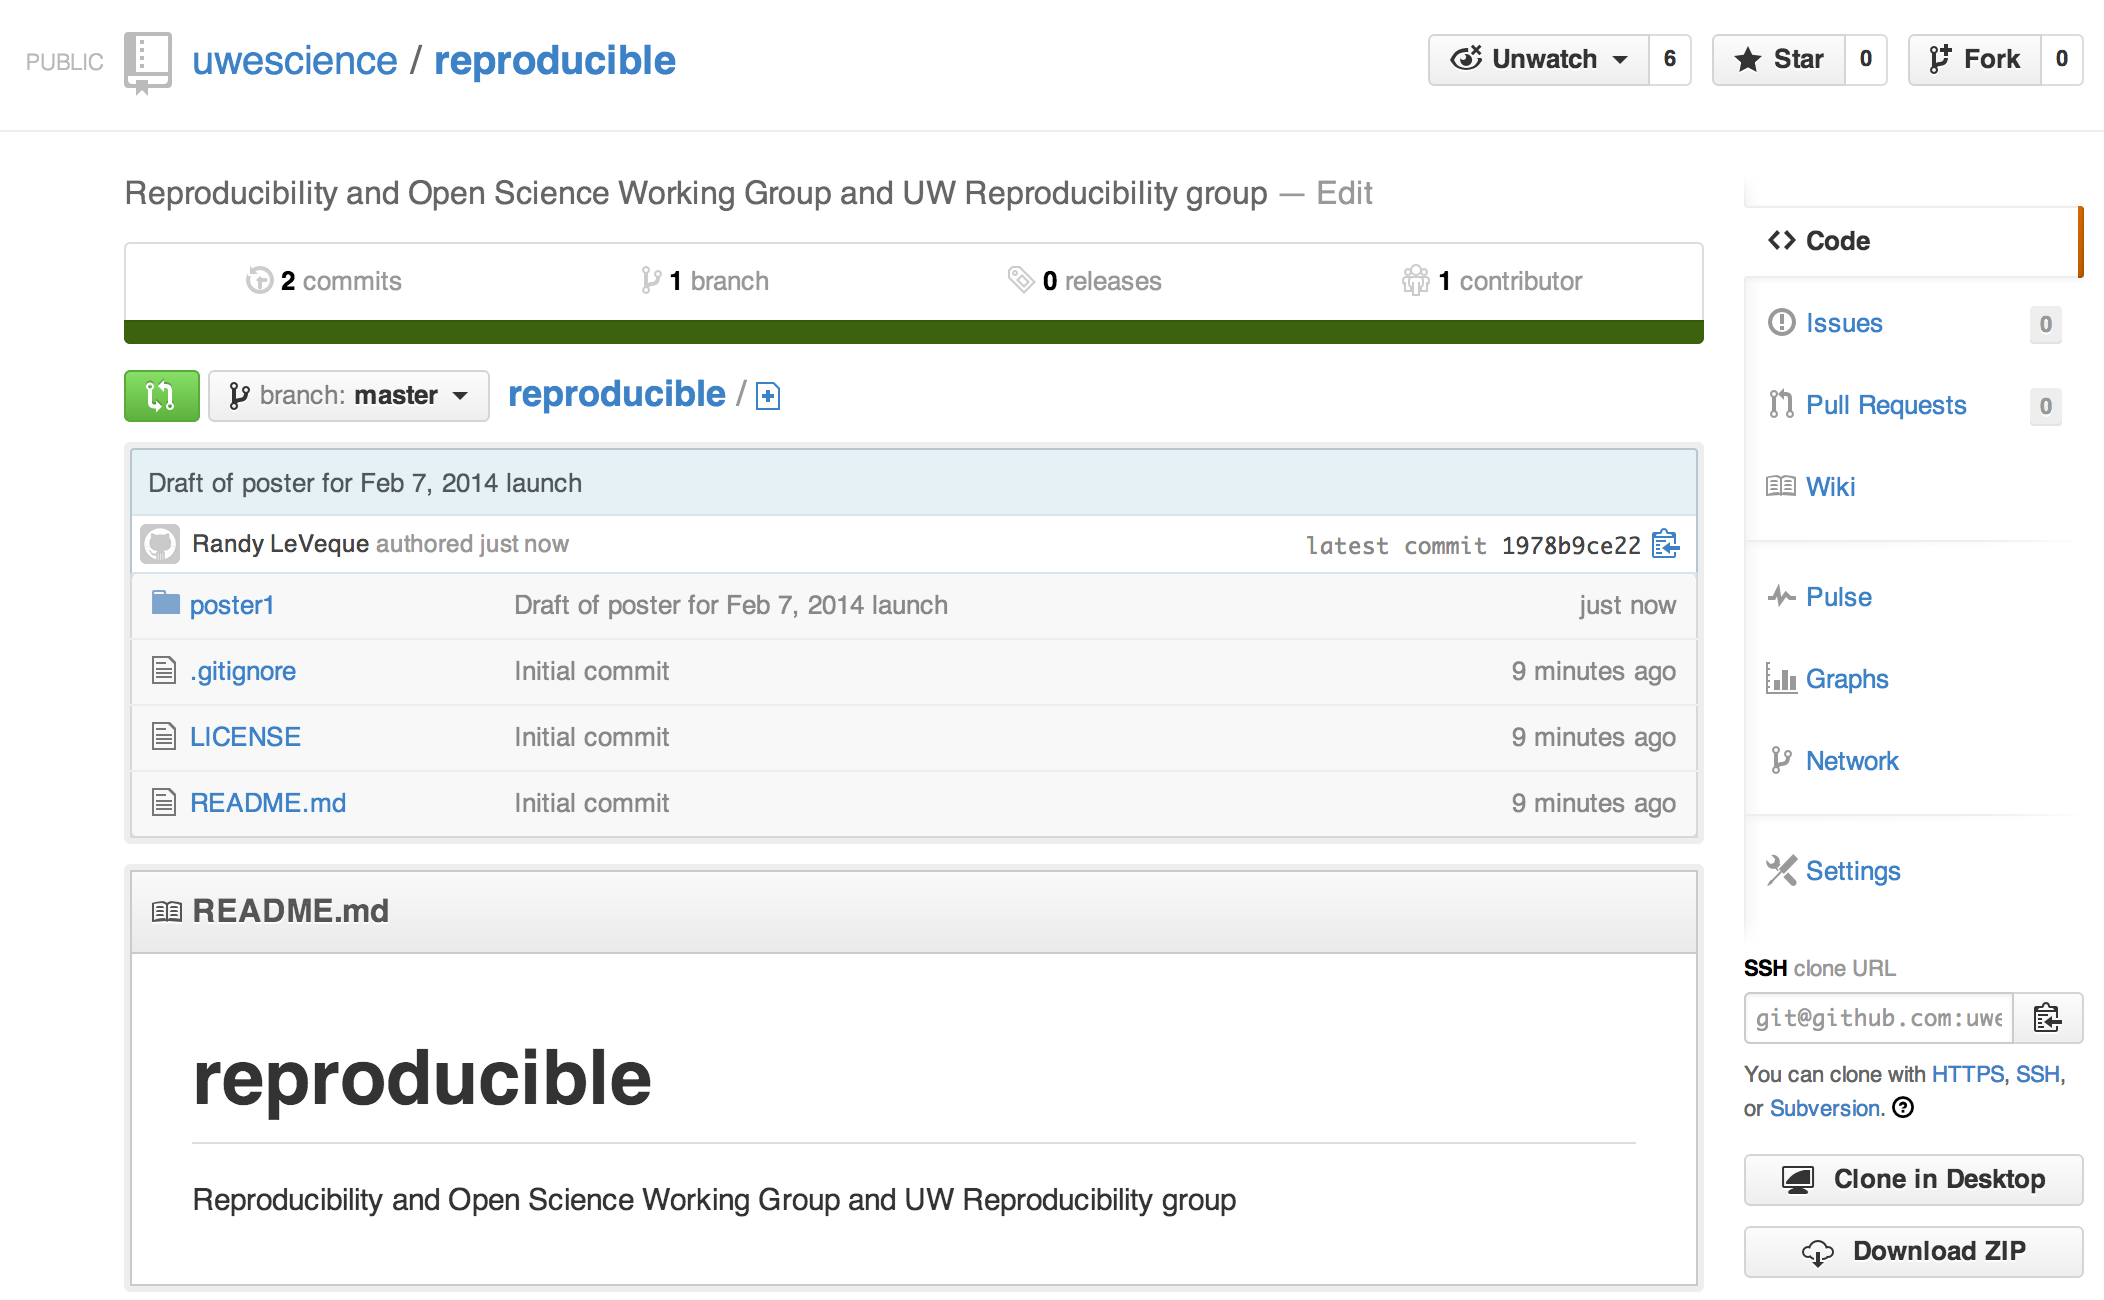
\includegraphics[width=5in]{github2.png} }

    \vskip 2ex
    Figshare for digital publishing / DOIs:\\
    \vskip 1ex \hskip 1.5in
    \framebox{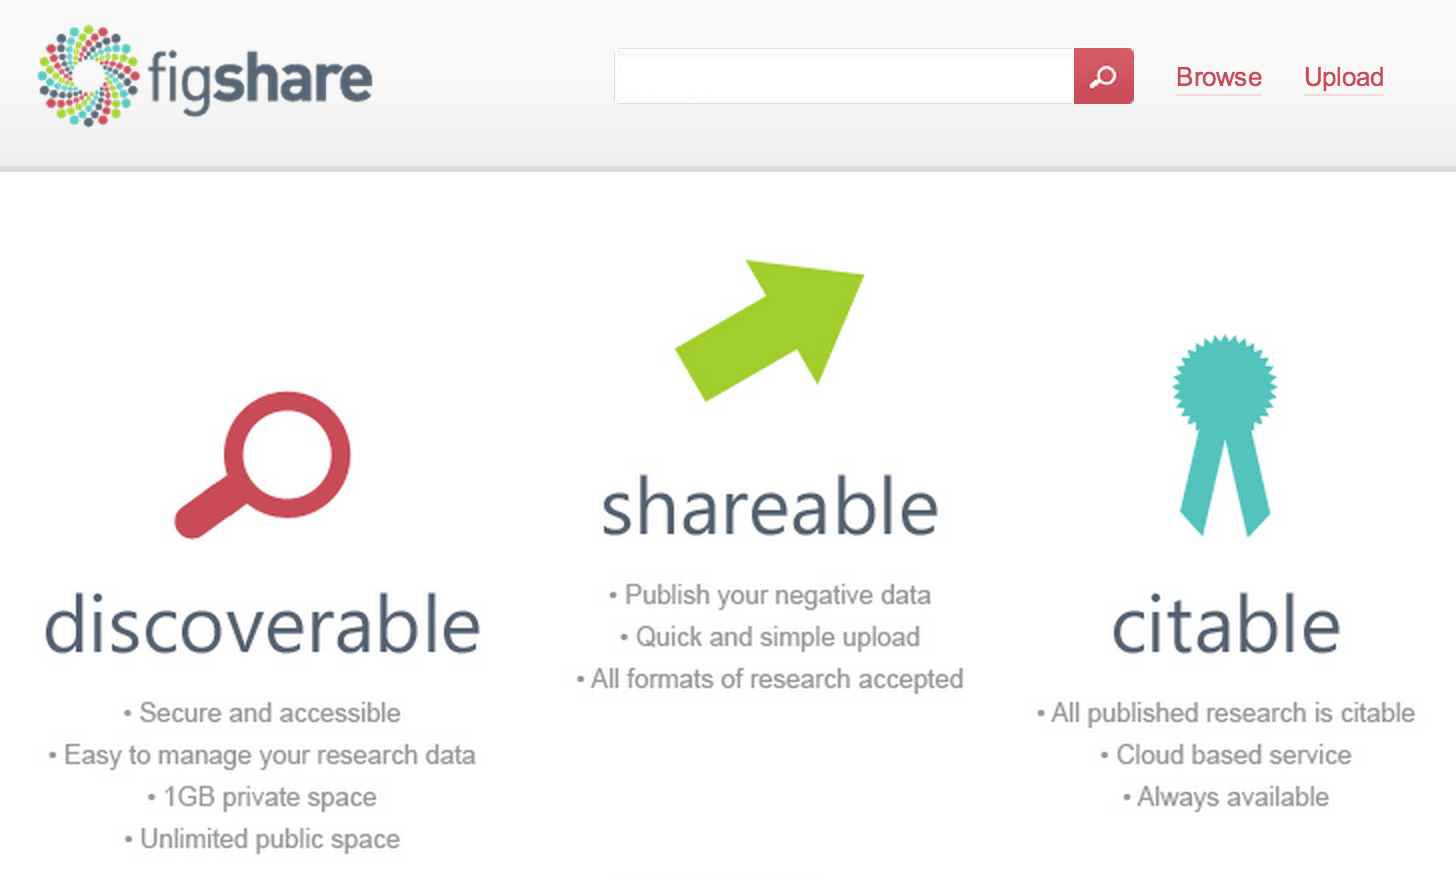
\includegraphics[width=5in]{figshare.png} }
    \vskip 2ex
    IPython notebooks:\\
    \vskip 1ex \hskip 1.5in
    \framebox{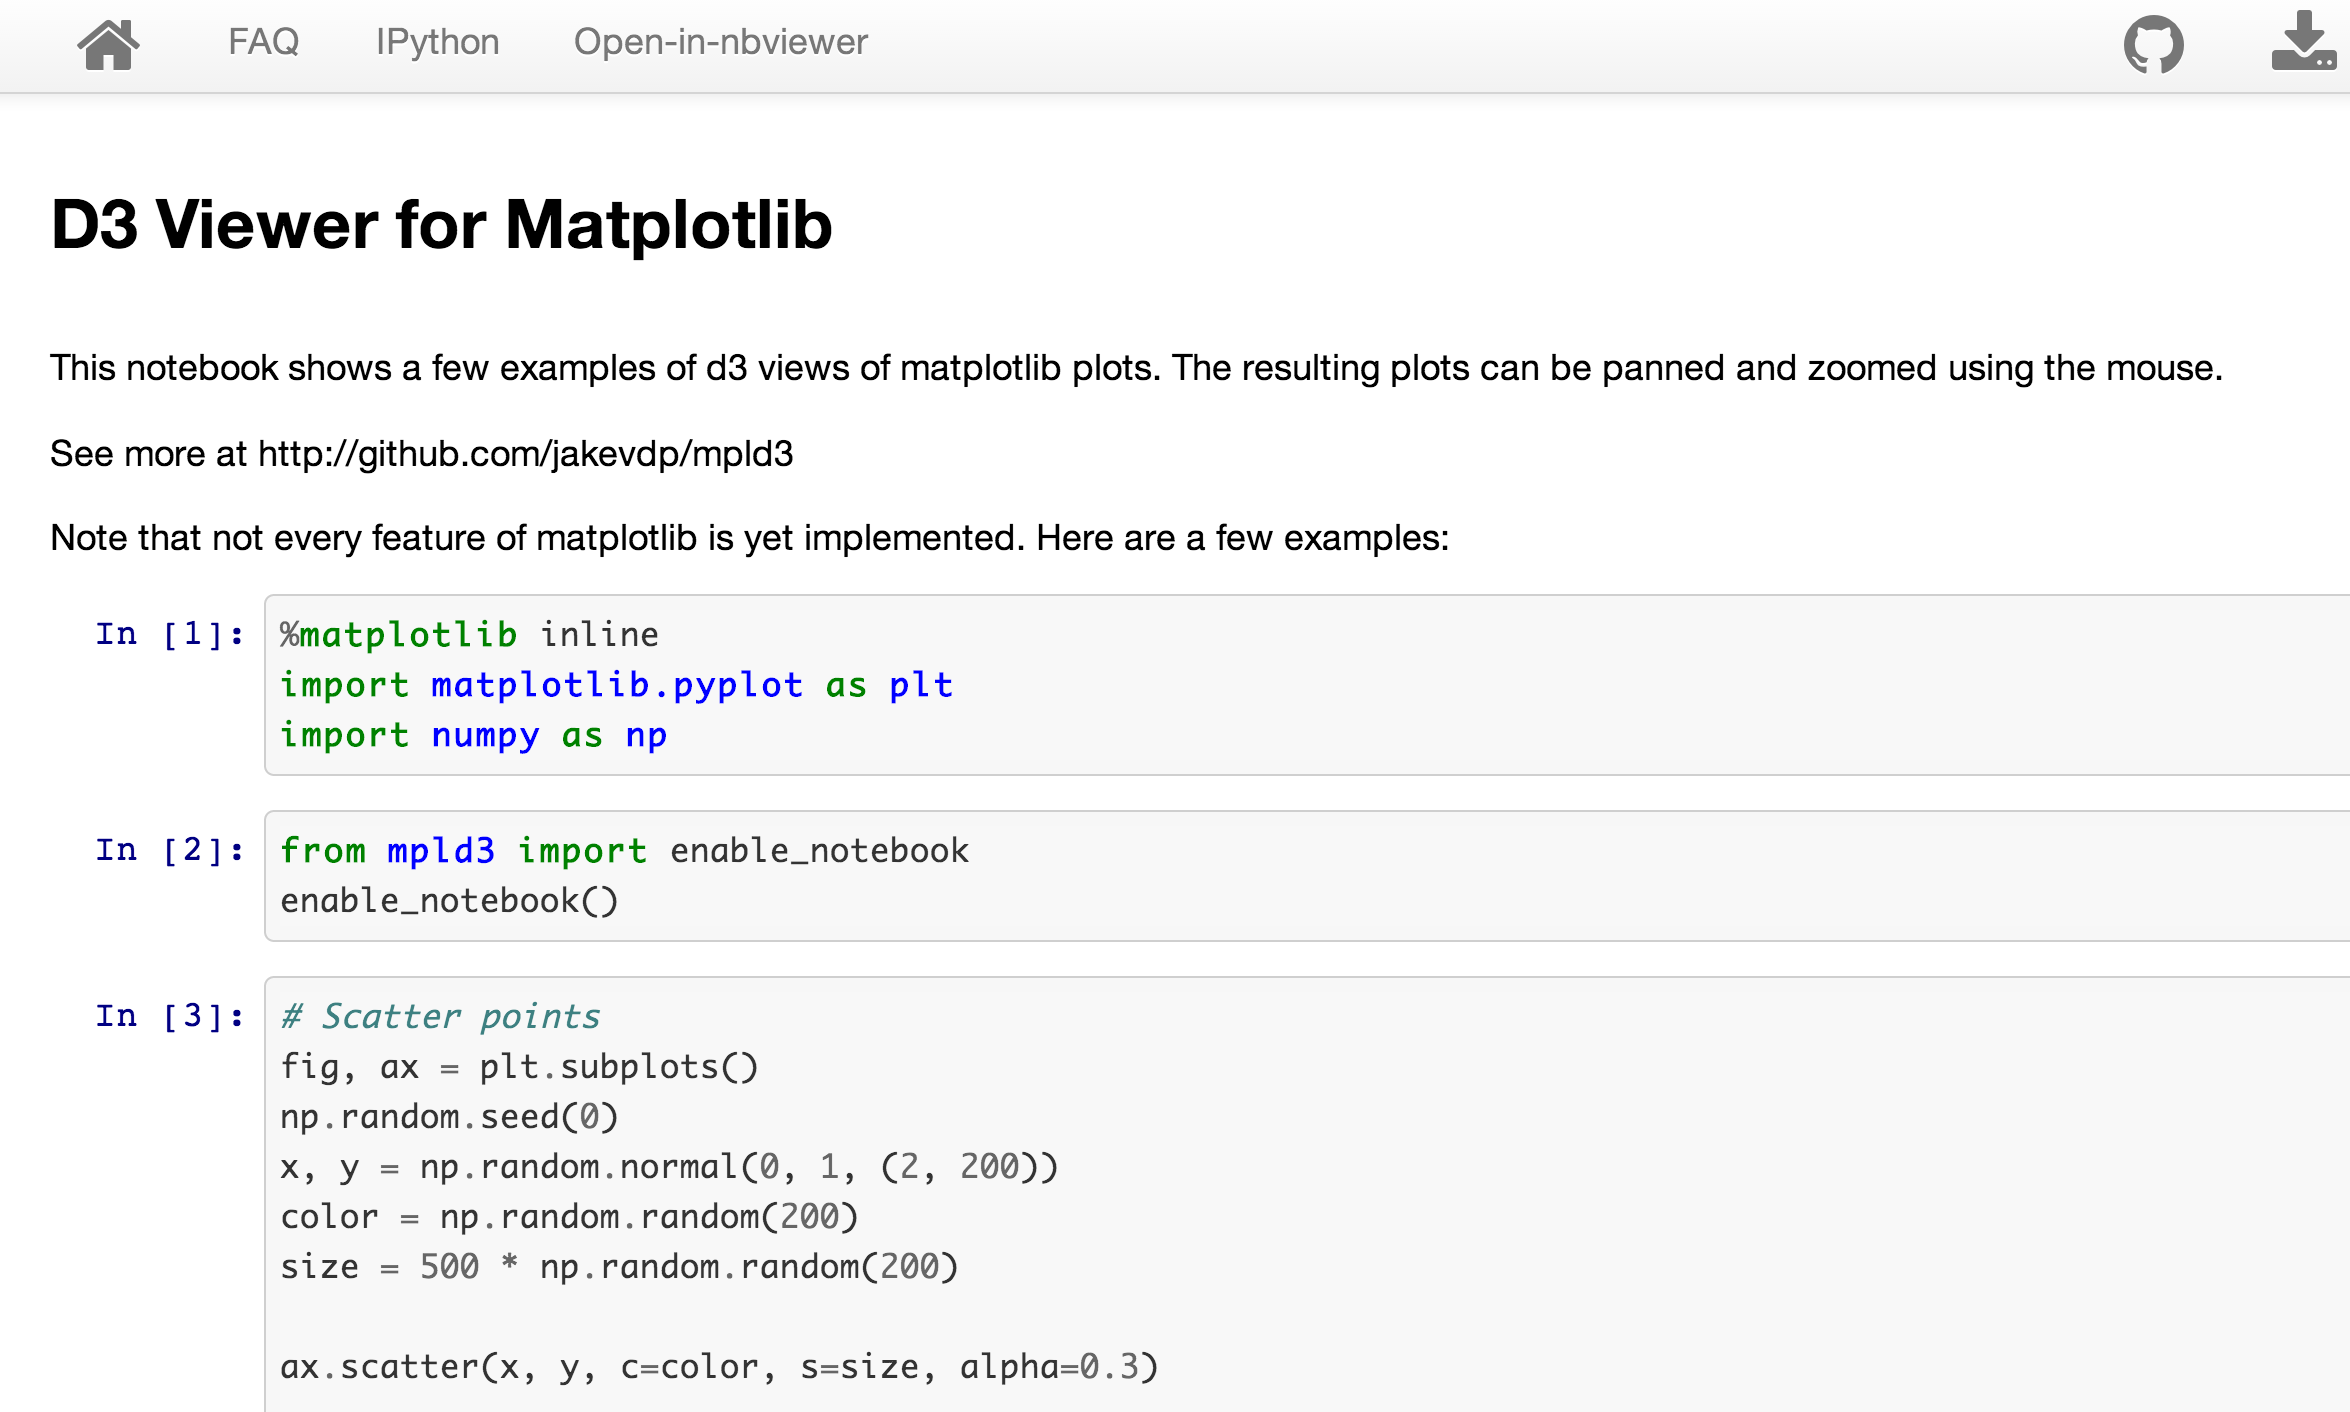
\includegraphics[width=5in]{ipython1.png} }
    \vskip 2ex
    SageMathCloud for sharing code:\\
    \vskip 1ex \hskip 1.5in
    \framebox{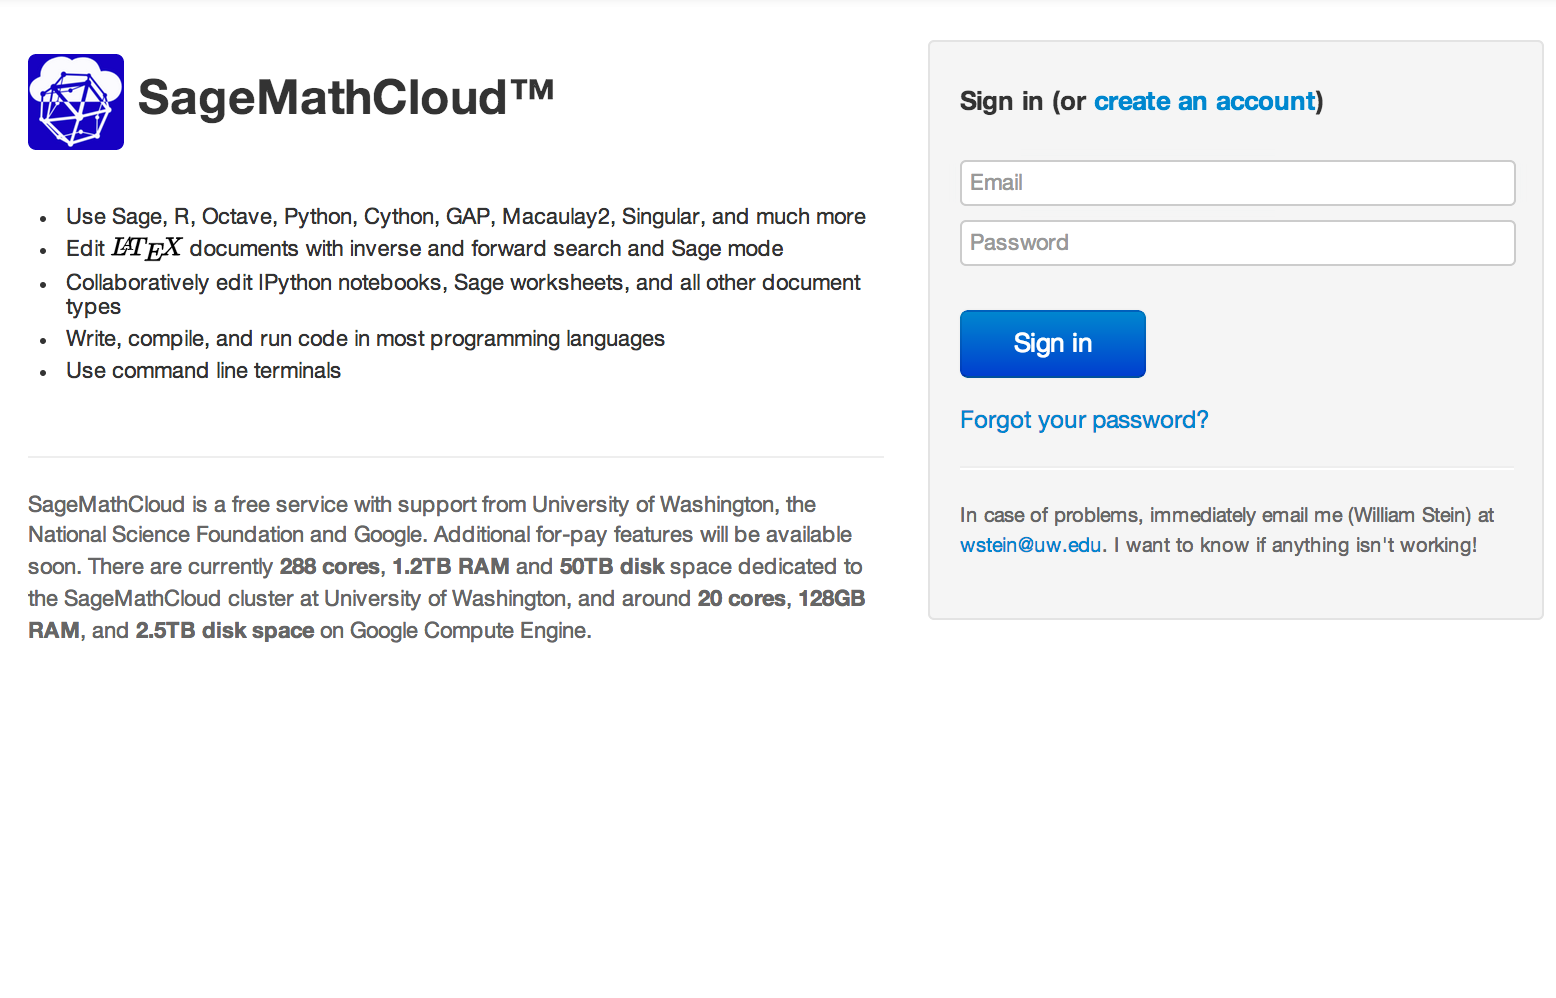
\includegraphics[width=5in]{sagemathcloud.png} }
    \vskip 2ex
    VisTrails for provenance tracking:\\
    \vskip 1ex \hskip 1.5in
    \framebox{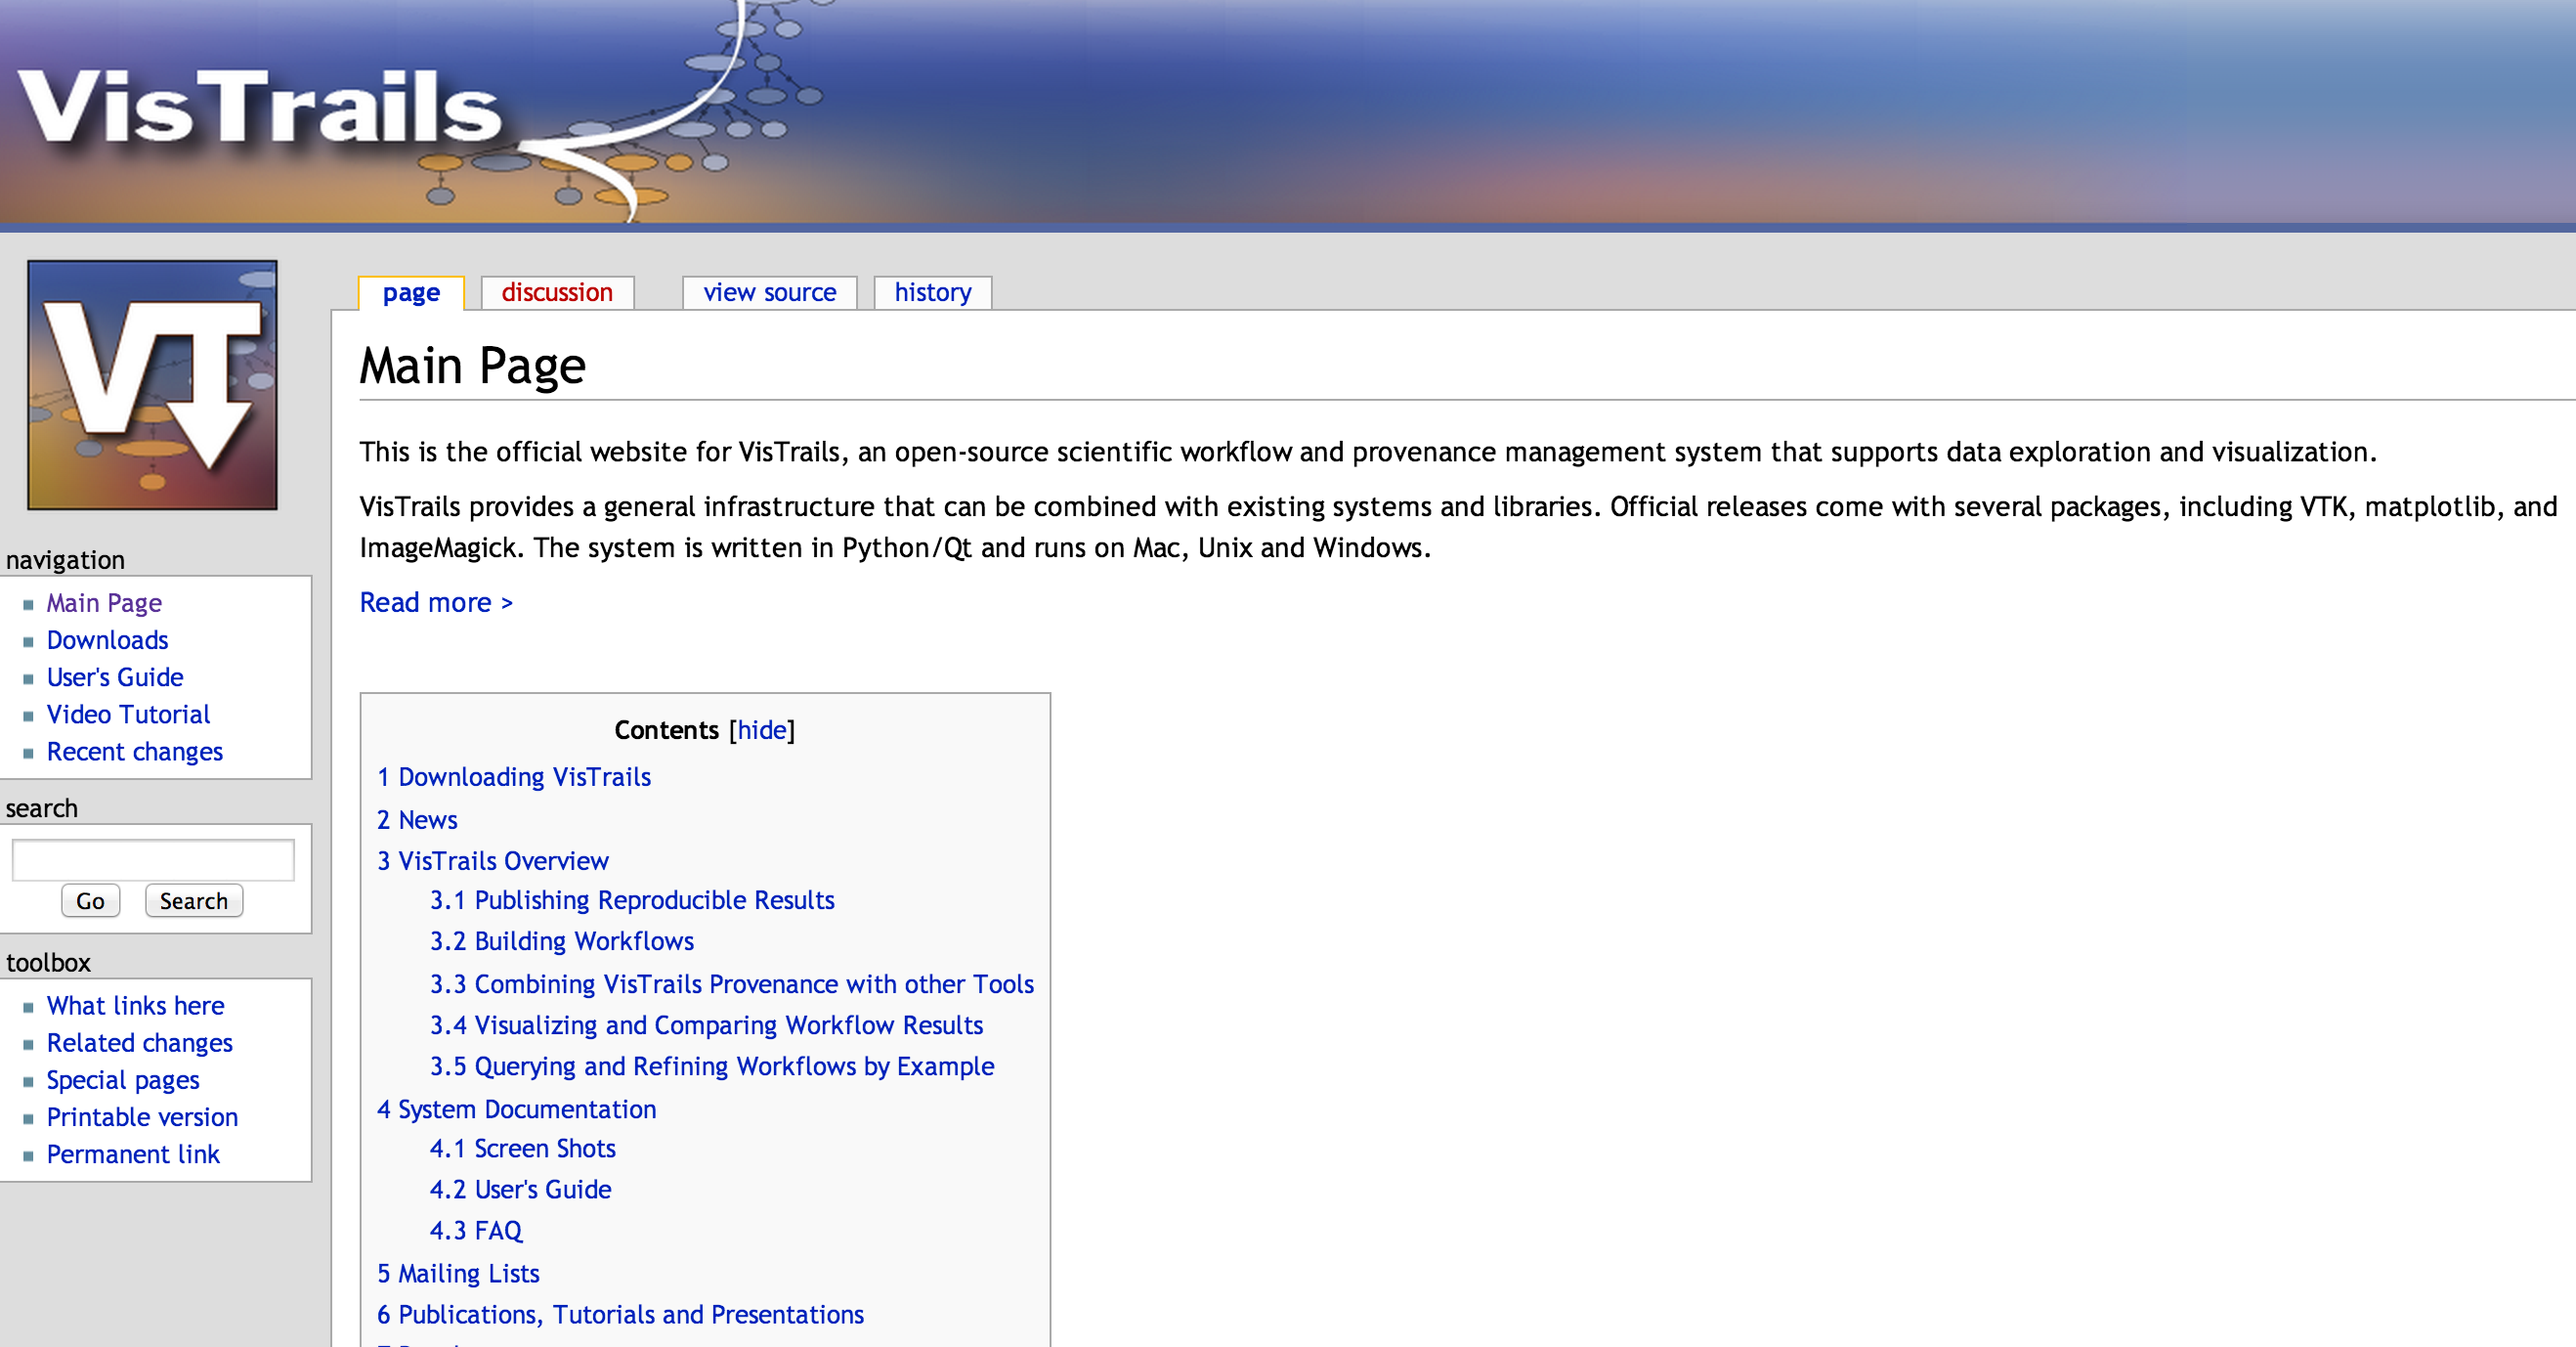
\includegraphics[width=5in]{vistrails.png} }
    \vskip 2ex
    Open Notebook Science:\\
    \vskip 1ex \hskip 1.5in
    \framebox{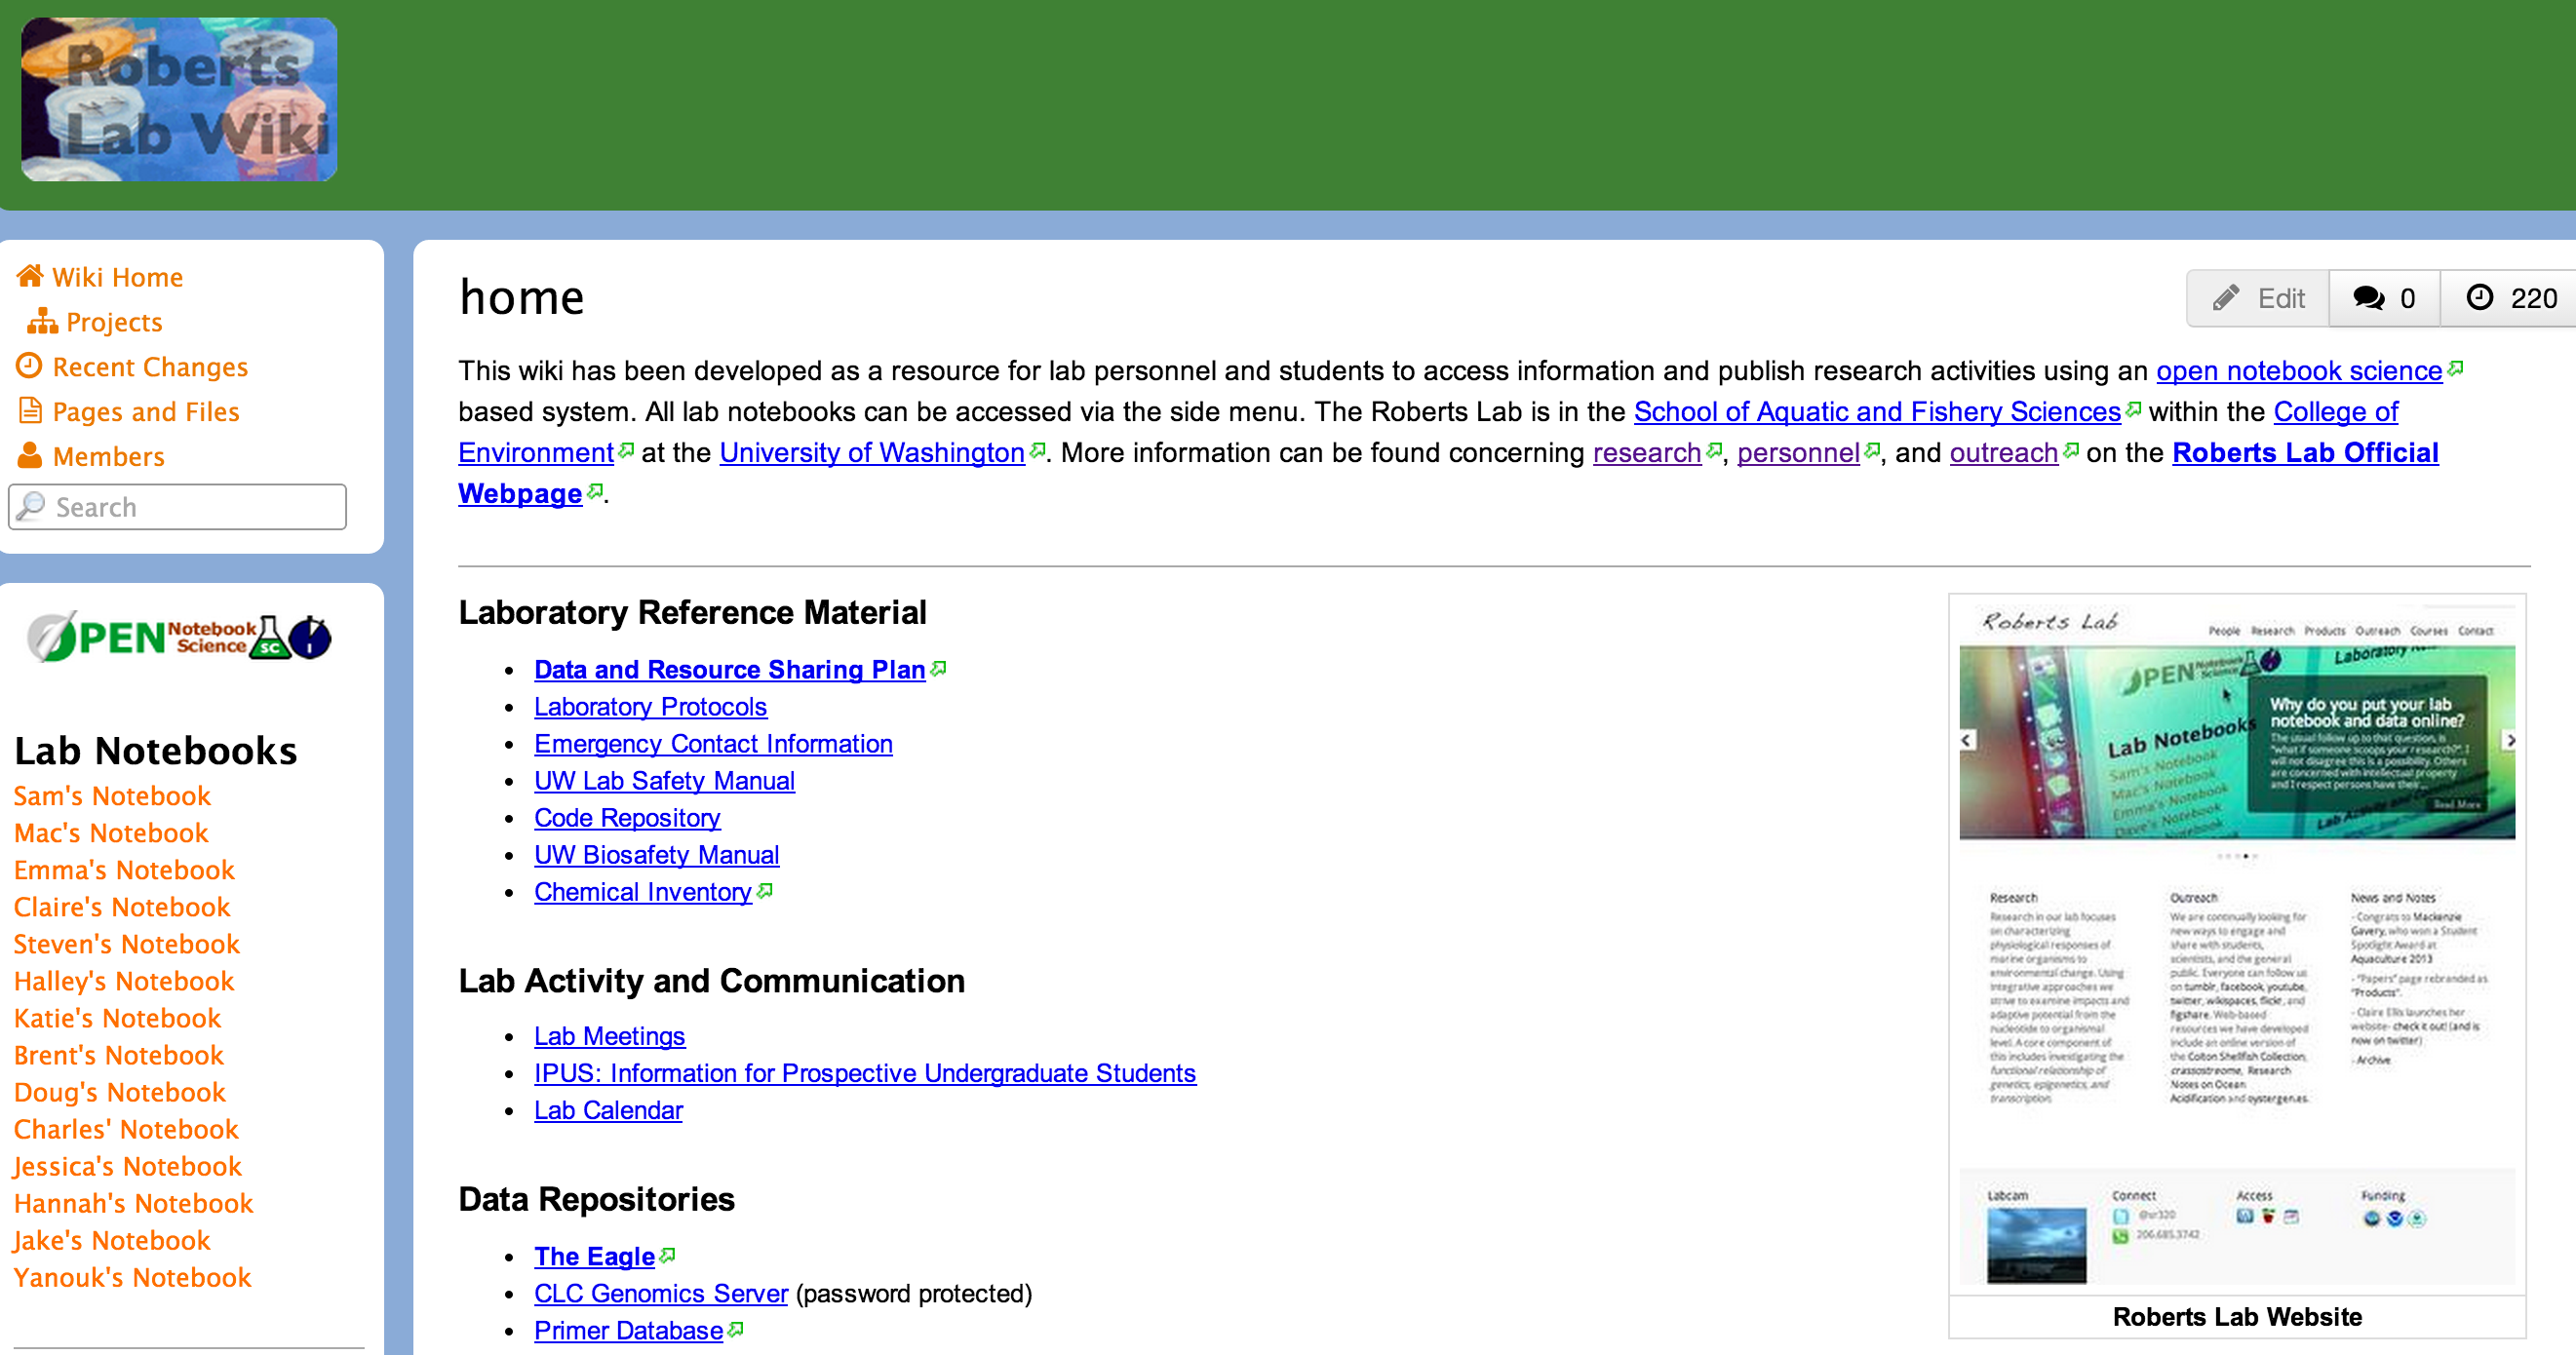
\includegraphics[width=5in]{roberts.png} }
    \vskip 2ex
    ~
    \end{column}
        
  %\begin{column}{\sepwid}\end{column} % empty spacer column

  \begin{column}{\onecolwid}       % COLUMN 3
        \begin{alertblock}{UW Reproducibility Group}
    \vskip 2ex
    \begin{center}
        All are welcome. 

        \vskip 1ex
        Meets at 2:30pm on the second Tuesday of each month.
       
        \vskip 1ex
         Join our mailing list for
        announcements and discussion.
    \end{center}
    
    ~
        \end{alertblock}
    \vskip 2cm
        \begin{alertblock}{Workshop --- May 8}
    \vskip 2ex
    \begin{center}
        A one-day workshop is scheduled on May 8, 2014. 
        \vskip 1ex
        Come to the morning sessions to learn more about the topic
        and/or join the break-out groups in the afternoon.
    \end{center}
    
    ~
        \end{alertblock}
    \vskip 2cm

    \begin{alertblock}{For more information} 
    \vskip2ex
    \begin{center}
    Visit the webpage below for more links and resources, including the
    schedule of the May 8 workshop and the mailing list for the UW
    Reproducibility group.
    \vskip 3ex

      {\sffamily http://escience.washington.edu/... \\ reproducible}
    \vskip 2ex
       
\includegraphics[width=2in]{qrcode.png} 

    ~
    \end{center}
    \end{alertblock}

    
\vskip 5ex

\includegraphics[width=9in]{MSlogos.png} 


  \end{column}

  %\begin{column}{\sepwid}\end{column}			% empty spacer column

 \end{columns}

\end{frame}
\end{document}
